\usepackage{xcolor}
\usepackage{afterpage}
\usepackage{pifont,mdframed}
\usepackage{multicol}
\usepackage[bottom]{footmisc}


\createsection{\Grader}{Grader di prova}

\renewcommand{\inputfile}{\texttt{stdin}}
\renewcommand{\outputfile}{\texttt{stdout}}
\makeatletter
\renewcommand{\this@inputfilename}{\texttt{stdin}}
\renewcommand{\this@outputfilename}{\texttt{stdout}}
\makeatother

% % % % % % % % % % % % % % % % % % % % % % % % % % % % % % % % % % % % % % % % % % %
% % % % % % % % % % % % % % % % % % % % % % % % % % % % % % % % % % % % % % % % % % %

Mojito, con l'aiuto di \emph{tutti} gli altri Jack Russell Terrier materani, ha
appena finito di appendere un lunghissimo striscione nella sala cerimonie
dell'\emph{IIS G.B. Pentasuglia} in vista della premiazione delle Olimpiadi di
Informatica. Mentre assapora il meritato riposo, Mojito nota che nella lunga
lista di sponsor è possibile identificare molti \textbf{pangrammi}: frasi in cui
vengono utilizzate tutte le lettere dell'alfabeto.

\begin{figure}[H]
  \centering
  \frame{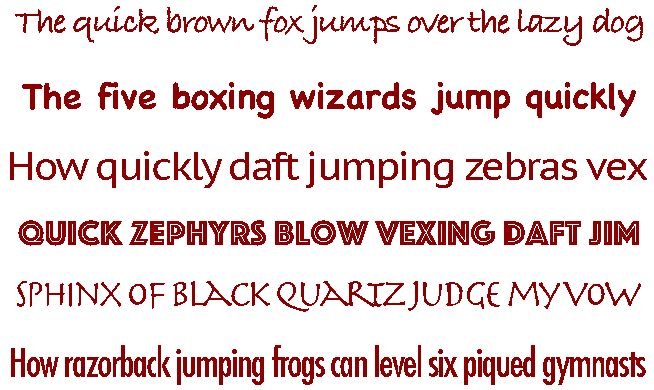
\includegraphics{pangram.pdf}}
  \caption{Una selezione di sei diversi pangrammi\footnotemark}
\end{figure}
\footnotetext{I pangrammi, oltre a stuzzicare Mojito, trovano effettivamente un
utilizzo nella vita reale. Ad esempio, in tipografia i pangrammi sono utili per
testare la resa grafica dei caratteri di stampa. Inoltre, telegrafare un
pangramma è un ottimo modo per chi vuole mettere alla prova la propria
conoscenza del codice Morse. Negli anni '80, anche lo scrittore Umberto Eco era
ossessionato dai pangrammi. Un pangramma eteroletterale in lingua italiana da
lui proposto fu il seguente:\\\phantom{xxxxxxxxxxxxxxxxxxxxxxxxxxxxxxxx}\emph{``Tv? Quiz, BR, FLM, DC... Oh, spenga!''}}

Ovviamente, non è difficile trovare pangrammi lunghi, mentre è molto più
difficile trovarne di corti. I pangrammi più corti possibili sono detti
\textbf{eteroletterali}, e usano ogni lettera \emph{esattamente una volta}:%
%
\begin{center}
  \texttt{Mr Jock TV quiz PhD bags few lynx}
\end{center}%
%
Purtroppo, non è detto che ci sia un pangramma così corto nello striscione. In
mancanza, Mojito si può accontentare di trovare i \textbf{pangrammi di lunghezza
minima} tra quelli presenti nello striscione.

Ispirato dalla scoperta, Mojito decide di organizzare una sfida con i suoi
aiutanti: a turno, ciascuno dei $\mathbf{46\,337}$ Jack Russell Terrier dovrà
mostrare agli altri un pangramma minimo. Per farlo, dovrà evidenziare
un'occorrenza di ogni lettera dell'alfabeto nello striscione, ovviamente in un
modo diverso da quanto gli altri hanno già fatto in precedenza. Prima di
iniziare la sfida, Mojito vuole capire in quanti modi diversi è possibile fare
questa ``evidenziazione''... altrimenti potrebbe rischiare di sfigurare!

Più precisamente, lo striscione riporta una stringa $V$ di $N$ caratteri,
ciascuno preso da un alfabeto di $K$ simboli.\footnote{Nello striscione non ci
sono solo lettere: ci possono essere numeri, caratteri speciali, emoji, il
simbolo di batman, \dots} I simboli sono rappresentati dai valori interi da $0$
a $K-1$. Una \emph{evidenziazione} associa ad ogni simbolo $j$ dell'alfabeto una
posizione $x_j$ nella stringa $V$ dove compare tale simbolo, quindi tale che
$V[x_j] = j$. Due evidenziazioni sono diverse se associano posizioni diverse
$x_j \neq x'_j$ ad almeno un simbolo $j$, anche se corrispondono allo stesso
pangramma. Un'evidenziazione è \emph{minima} se individua un pangramma minimo
(cioè, se la massima differenza $x_j - x_i$ tra le posizioni di due occorrenze è
minima possibile). Mojito vuole contare quante evidenziazioni minime diverse
esistono, \textbf{modulo} $\mathbf{46\,337}$: aiutalo tu!

% % % % % % % % % % % % % % % % % % % % % % % % % % % % % % % % % % % % % % % % % % %
% % % % % % % % % % % % % % % % % % % % % % % % % % % % % % % % % % % % % % % % % % %


\Implementation

\begin{danger}
  È importante usare sempre il modulo dopo una somma perché i valori intermedi
  generati possono richiedere più di 32 bit. Quando si cerca un risultato modulo
  $M$, suggeriamo di sfruttare il fatto che ($A$ + $B$ + $C$) modulo $M$ =
  ((($A$ + $B$) modulo $M$) + $C$) modulo $M$. La stessa cosa vale per la
  moltiplicazione. In questo modo, i risultati intermedi restano sempre modulo
  $M$ e possono essere mantenuti in una variabile intera.
\end{danger}

Dovrai sottoporre un unico file, con estensione \texttt{.c} o \texttt{.cpp}.

\begin{warning}
Tra gli allegati a questo task troverai dei template \texttt{pangramma.c} e
\texttt{pangramma.cpp} con un esempio di implementazione.
\end{warning}

Dovrai implementare la seguente funzione:

\begin{center}\begin{tabularx}{\textwidth}{|c|X|}
\hline
C    & \verb|int conta(int N, int K, int* V);|\\
C++  & \verb|int conta(int N, int K, vector<int>& V);|\\
\hline
\end{tabularx}\end{center}

\begin{itemize}[nolistsep]
  \item L'intero $N$ rappresenta la lunghezza dell'array \texttt{V}, ovvero il
        numero totale di lettere nello striscione.
  \item L'intero $K$ rappresenta il numero di simboli diversi che sono presenti nell'alfabeto.
  \item L'array \texttt{V}, indicizzato da $0$ a $N-1$, indica il simbolo
        contenuto in ciascuna posizione.
  \item La funzione deve restituire il numero di evidenziazioni minime diverse modulo $46\,337$.
\end{itemize}

\medskip

Il grader chiamerà la funzione \texttt{conta} e ne stamperà il valore restituito
sul file di output.

% % % % % % % % % % % % % % % % % % % % % % % % % % % % % % % % % % % % % % % % % % %
% % % % % % % % % % % % % % % % % % % % % % % % % % % % % % % % % % % % % % % % % % %


\Grader

Nella directory relativa a questo problema è presente una versione semplificata
del grader usato durante la correzione, che puoi usare per testare le tue
soluzioni in locale. Il grader di esempio legge i dati da \inputfile{}, chiama
la funzione che devi implementare e scrive su \outputfile{}, secondo il seguente
formato.

Il file di input è composto da due righe, contenenti:
\begin{itemize}[nolistsep,itemsep=2mm]
\item Riga $1$: due interi $N$ e $K$.
\item Riga $2$: $N$ interi \texttt{V[$i$]} per $i = 0\ldots N-1$.
\end{itemize}

Il file di output è composto da un'unica riga, contenente il valore restituito
dalla funzione \texttt{conta}.

% % % % % % % % % % % % % % % % % % % % % % % % % % % % % % % % % % % % % % % % % % %
% % % % % % % % % % % % % % % % % % % % % % % % % % % % % % % % % % % % % % % % % % %


\Constraints

\begin{itemize}[nolistsep, itemsep=2mm]
    \item $1 \le K \le N \le 1\,000\,000$.
    \item $0 \le$ \texttt{V[$i$]} $\le K-1$ per $i = 0\dots N-1$.
    \item Tutti i simboli compaiono almeno una volta nella stringa.
\end{itemize}

% % % % % % % % % % % % % % % % % % % % % % % % % % % % % % % % % % % % % % % % % % %
% % % % % % % % % % % % % % % % % % % % % % % % % % % % % % % % % % % % % % % % % % %


\Scoring

Il tuo programma verrà testato su diversi test case raggruppati in subtask.
Per ottenere il punteggio relativo ad un subtask, è necessario risolvere correttamente tutti i test che lo compongono.

\begin{itemize}[nolistsep,itemsep=2mm]
  \item \textbf{\makebox[2.3cm][l]{Subtask \phantom{1}1} [\phantom{1}0 punti]}: Casi d'esempio.
  \item \textbf{\makebox[2.3cm][l]{Subtask \phantom{1}2} [\phantom{1}5 punti]}: $K = 2$.
  \item \textbf{\makebox[2.3cm][l]{Subtask \phantom{1}3} [\phantom{1}7 punti]}: $N \le 30$.
  \item \textbf{\makebox[2.3cm][l]{Subtask \phantom{1}4} [14           punti]}: $N \le 300$.
  \item \textbf{\makebox[2.3cm][l]{Subtask \phantom{1}5} [13           punti]}: $N \le 5000$.
  \item \textbf{\makebox[2.3cm][l]{Subtask \phantom{1}6} [12           punti]}: Nello striscione c'è almeno un pangramma \textit{eteroletterale}.
  \item \textbf{\makebox[2.3cm][l]{Subtask \phantom{1}7} [11           punti]}: Il pangramma minimo è lungo al massimo $60$.
  \item \textbf{\makebox[2.3cm][l]{Subtask \phantom{1}8} [10           punti]}: Il numero di evidenziazioni minime è al massimo $10^9$.
  \item \textbf{\makebox[2.3cm][l]{Subtask \phantom{1}9} [\phantom{1}9 punti]}: $N \le 500\,000$.
  \item \textbf{\makebox[2.3cm][l]{Subtask           10} [10           punti]}: Nessuna limitazione specifica.
  \item \textbf{\makebox[2.3cm][l]{Subtask           11} [\phantom{1}7 punti]}: \raisebox{0.05cm}{{\fontencoding{U}\fontfamily{futs}\selectfont\char 66\relax}}\emph{Caso speciale:} $1\,000\,000 \le K \le N \le 5\,000\,000$.
  \item \textbf{\makebox[2.3cm][l]{Subtask           12} [\phantom{1}2 punti]}: \raisebox{0.05cm}{{\fontencoding{U}\fontfamily{futs}\selectfont\char 66\relax}}\emph{Caso speciale:} $5\,000\,000 \le K \le N \le 9\,000\,000$.
\end{itemize}

% % % % % % % % % % % % % % % % % % % % % % % % % % % % % % % % % % % % % % % % % % %
% % % % % % % % % % % % % % % % % % % % % % % % % % % % % % % % % % % % % % % % % % %


\Examples

\begin{example}
\exmpfile{pangramma.input0.txt}{pangramma.output0.txt}%
\exmpfile{pangramma.input1.txt}{pangramma.output1.txt}%
\exmpfile{pangramma.input2.txt}{pangramma.output2.txt}%
\exmpfile{pangramma.input3.txt}{pangramma.output3.txt}%
\end{example}

% % % % % % % % % % % % % % % % % % % % % % % % % % % % % % % % % % % % % % % % % % %
% % % % % % % % % % % % % % % % % % % % % % % % % % % % % % % % % % % % % % % % % % %


\Explanation

Nel \textbf{primo caso di esempio} sono presenti due pangrammi minimi, che sono anche eteroletterali:%
\begin{center}
  \tt
  \begin{tikzpicture}
    \node[draw,dashed] at (-0.95, 0) {\colorbox{yellow!90}{2},\colorbox{yellow!90}{0},\colorbox{yellow!90}{1}};
    \node[text] at (0.95, -0.03) {, 1, 2, 0};
  \end{tikzpicture}
  \quad
  \begin{tikzpicture}
    \node[text] at (-0.92, -0.03) {2, 0, 1,};
    \node[draw,dashed] at (0.92, 0) {\colorbox{yellow!90}{1},\colorbox{yellow!90}{2},\colorbox{yellow!90}{0}};
  \end{tikzpicture}
\end{center}

Ci sono anche altri pangrammi più lunghi, che però non vanno contati:%
\begin{center}
  \tt
  \begin{tikzpicture}
    \node[text] at (-1.51, 0) {2,};
    \node[draw,dashed] at (0, 0) {0, 1, 1, 2};
    \node[text] at (1.51, 0) {, 0};
  \end{tikzpicture}
\end{center}
In totale, ci sono quindi $\mathbf{2}$ modi diversi per evidenziare un pangramma di lunghezza minima.

Nel \textbf{secondo caso di esempio}, sono di nuovo presenti due pangrammi minimi, anche se non sono eteroletterali, per un totale di $\mathbf{4}$ evidenziazioni minime:%
\begin{center}
  \tt
  \begin{tikzpicture}
    \node[draw,dashed] at (-1.2, 0) {\colorbox{yellow!90}{0},\,\colorbox{yellow!90}{1}, 1,\,\colorbox{yellow!90}{2}};
    \node[text] at (1.1, -0.03) {, 1, 1, 0};
  \end{tikzpicture}
  \quad
  \begin{tikzpicture}
    \node[text] at (-1.1, -0.03) {0, 1, 1, };
    \node[draw,dashed] at (1.1, 0) {\colorbox{yellow!90}{2},\,\colorbox{yellow!90}{1}, 1,\,\colorbox{yellow!90}{0}};
  \end{tikzpicture}

  \begin{tikzpicture}
    \node[draw,dashed] at (-1.2, 0) {\colorbox{yellow!90}{0}, 1,\,\colorbox{yellow!90}{1},\,\colorbox{yellow!90}{2}};
    \node[text] at (1.1, -0.03) {, 1, 1, 0};
  \end{tikzpicture}
  \quad
  \begin{tikzpicture}
    \node[text] at (-1.1, -0.03) {0, 1, 1, };
    \node[draw,dashed] at (1.1, 0) {\colorbox{yellow!90}{2}, 1,\,\colorbox{yellow!90}{1},\,\colorbox{yellow!90}{0}};
  \end{tikzpicture}
\end{center}

Nel \textbf{terzo caso di esempio} c'è un unico pangramma eteroletterale, al
centro, e quindi c'è una sola evidenziazione minima.

Nel \textbf{quarto caso di esempio} ci sono 2 pangrammi minimi, rispettivamente
con $6$ e con $4$ evidenziazioni minime, per un totale di $10$.
